% This manual is under CC BY-NC 4.0 license
% Copyright 2015 Danila Vella and Dario Di Silvestre

\documentclass[a4paper,14pt]{extarticle} 

\usepackage[british,UKenglish,USenglish,english,american]{babel}
%\usepackage[utf8]{inputenc} % Consente l'uso caratteri accentati italiani 
%\usepackage{cite} % Per inserire le citazioni
\usepackage{authblk} % Per inserire autori diversi del lavoro
\usepackage{comment} % Permette di inserire dei commenti
\usepackage{textgreek} % Lettere greche in text mode
\usepackage{siunitx} % Per inserire numeri e unità di misura
\usepackage[section]{placeins}

\usepackage{graphicx} % Inserire figure
\graphicspath{ {images/} }



\DeclareGraphicsExtensions{.png,.jpg}
\begin{document}

%\bibliographystyle{vancouver}
\begin{titlepage}
\begin{center}
\textsc{\LARGE Supplementary information}\\[3cm]
\textsc{\huge  EPPI manual}\\[1.5cm]
\end{center}
\end{titlepage}

%---------------------------------------------------------------------
% Danila
\section{Getting start}
EPPI is a software to process proteomic data obtained by mass-spectrometry analysis, with the aim to identify proteotypic peptides (PTPs). The data processing is composed by several steps linked between them. The steps will be described according the logical sequence of data elaboration.\\
The first step to use EPPI is to create a new project or to open an existing one, using the Project menu (\figurename~\ref{fig:project}).

\begin{figure}[htbp]
\centering
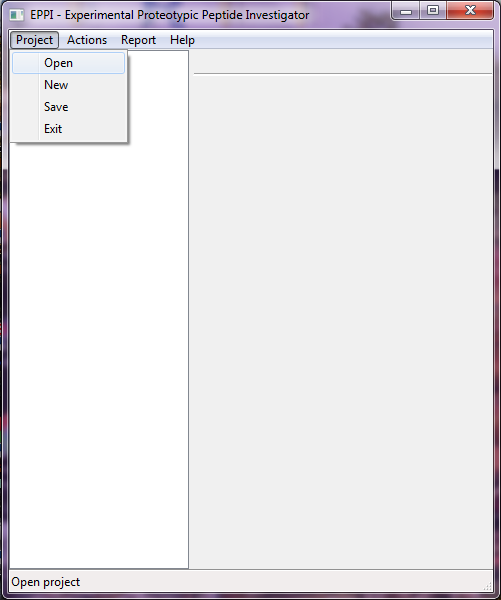
\includegraphics[scale=0.5]{open}%
\hspace{5mm}
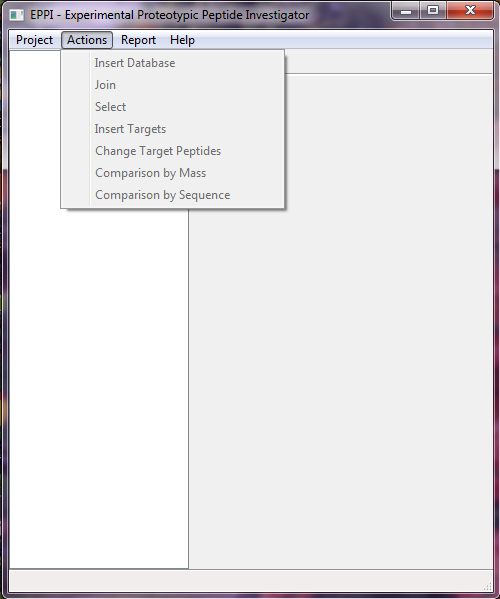
\includegraphics[scale=0.5]{Action}
\caption{Left: Project menu. Right: Action menu.}\label{fig:project}

\end{figure}

%Danila
 

\section{Inserting and pre-processing data: Join function}

Main functions are reported in Action menu (\figurename~\ref{fig:project}).
The Join function permits to insert input data through a folder containing them. EPPI accepts files produced by Bioworks 3.3.1, Discoverer 1.4, Mascot and PRIDE. XML, XLS and mzIdentML formats are accepted (\figurename~\ref{fig:join}). 

\begin{figure}[htbp]
\begin{center}
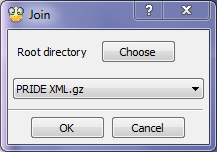
\includegraphics[scale=0.8]{EPPI_join}%
\hspace{5mm}
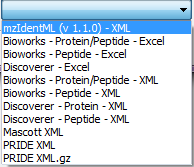
\includegraphics[scale=0.8]{formatFile}
\caption{Left: Join function. Right: file formats EPPI is able to accept in input.}\label{fig:join}
\end{center}
\end{figure}

After data are loaded, EPPI merges the input files and for each identified peptide and protein it calculates the Identification Frequency (IF). The results of this processing are shown in all\_peptides table, reported in \figurename~\ref{fig:allp}.

\begin{figure}[ht]
\begin{center}
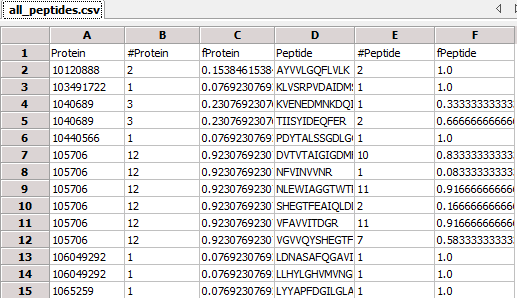
\includegraphics[scale=0.8]{Eppi_all_peptides}
\caption{All\_peptides table (result of Join function). Protein: identifier number of a given protein; \#Protein/\#Peptide: number of times that a given protein/peptide occurs in the input files; Peptide: peptide sequence; fProtein/fPeptide: identification frequency of proteins/peptides.}\label{fig:allp}
\end{center}
\end{figure}

\section{Selecting PTPs candidates}
The output data of previous step (see \figurename~\ref{fig:allp}) may be further processed using the “Select” function, that permits to filter the identification frequency (IF) values and the extraction of proteins and peptides with the best occurrence (\figurename~\ref{fig:select}).
 

 
\begin{figure}[ht]
\begin{center}
\includegraphics[scale=0.8]{EPPI_select.png}	
\caption{Select function. Interface to introduce threshold values concerning the identification frequency (IF) of proteins and peptides.}\label{fig:select}
\end{center}
\end{figure}

The peptides with IF overtaking the applied thresholds are considered "best". The result of this selection is shown in best\_peptides table (\figurename~\ref{fig:best}), which has the same attributes of all\_peptides table (see \figurename~\ref{fig:allp}) but it contains only the peptides defined best. 
\begin{figure}[ht]
\begin{center}
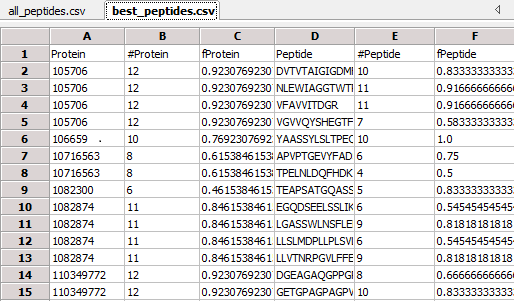
\includegraphics[scale=0.8]{Eppi_best_peptides.png}	
\caption{Best\_peptides table, result of Select function. Protein: identifier number of a given best protein; \#Protein/\#Peptide: number of times that a given best protein/peptide occurs in the input files; Peptide: sequence of a best peptide; fProtein/fPeptide: identification frequency of best proteins/peptides.}\label{fig:best}
\end{center}
\end{figure}
 
Furthermore, by selecting Histogram and Scatter Plot option (\figurename~\ref{fig:select}) two graphics that resume data will be create (\figurename~\ref{fig:graphics}).
 


\begin{figure}[ht]
\begin{center}
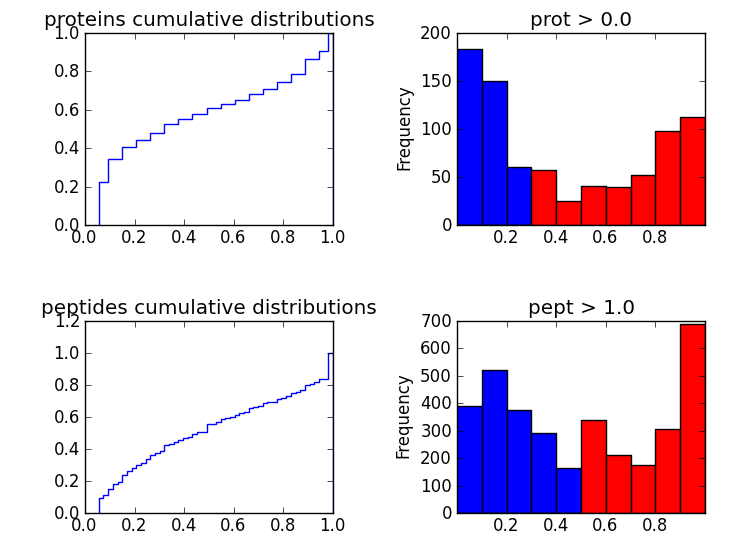
\includegraphics[scale=0.4]{pie_hist.png}%
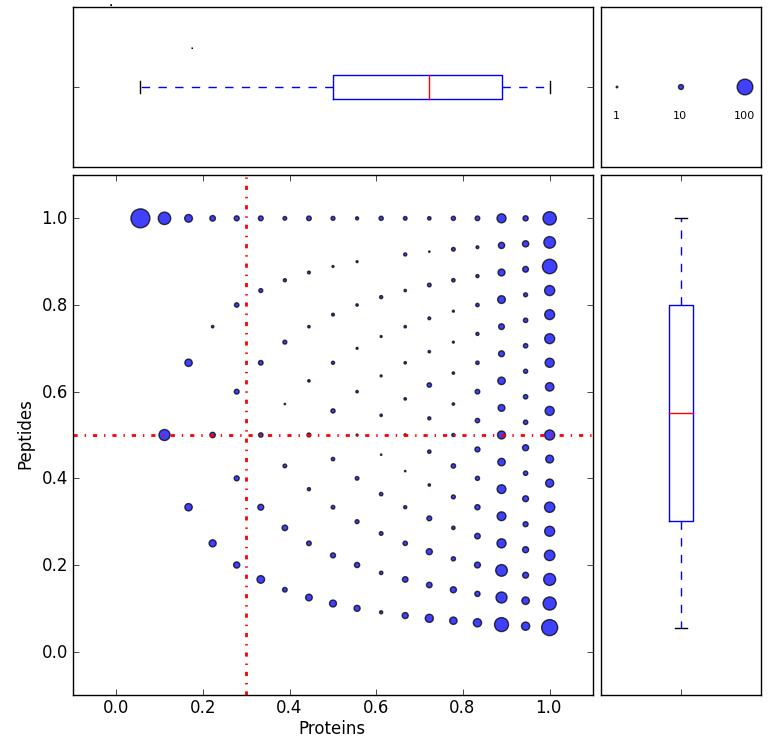
\includegraphics[scale=0.3]{scatter.png}
\caption{Right: Identification Frequency(IF) distribution of proteins and peptides. Left: scatter plot representing the number (by point width) of peptides with a given IF versus the IF of the corresponding parent protein.}\label{fig:graphics}
\end{center}
\end{figure}
\section{Inserting background proteome}


The Insert Database function allows to insert a reference database (fasta format) and to set some parameters for processing the experimental data (\figurename~\ref{fig:database}). The user has to set a digestion enzyme, to produce a reference peptidome, the miss cleavage value and a tolerance delta mass. In this way, selected best peptides will be compared against a database containing the background proteome to be defined proteotypic.
 
\begin{figure}[htbp]
\begin{center}
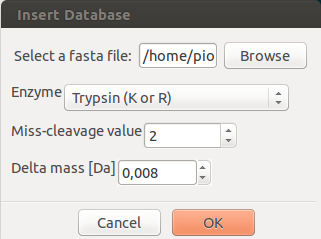
\includegraphics[scale=0.8]{EPPI_insert_database}
\caption{Insert Database function. By means of this window, it is possibile to introduce a protein database (.fasta format), that will be processed to create a virtual peptidome used to calculate the peptide uniqueness by sequence and molecular weight}.\label{fig:database}
\end{center}
\end{figure}

\section{Inserting target proteins}

The Insert Target function allows to insert the target proteins for which the user want to retrieve PTPs. The user can process all the identified peptides or only those defined "best" (Peptide Set option in \figurename~\ref{fig:targetProt}). To set the target proteins, the user can directly insert a list of protein identifiers or through an Excel file (\figurename~\ref{fig:targetProt}).

\begin{figure}[htbp]
\begin{center}
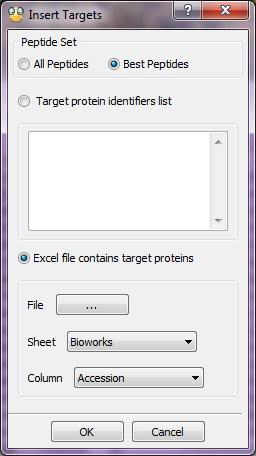
\includegraphics[scale=0.8]{Eppi_insert_target}
\caption{Insert Targets function. By means of this window, the users may insert target protein identifiers to retrieve the related best peptides, and to calculate their uniqueness. Since not all proteins could be associated to a best peptide, it is possible to perform this computation by considering all identified peptides (All Peptides). }\label{fig:targetProt}
\end{center}
\end{figure}

Following this function, EPPI returns two tables: peptides\_in\_targets (\label{fig:targetPepTable}) and target\_proteins\_list (\figurename~\ref{fig:targetProtTable}). Peptides\_in\_targets table reports if the peptide is considered best or not, while the target\_proteins\_list table reports for each target protein how many peptides were globally found in analysis and how many of them are considered best.

\begin{figure}[htbp]
\begin{center}
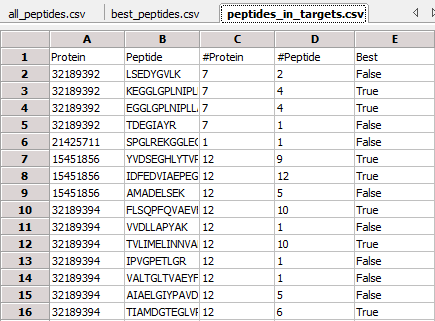
\includegraphics[scale=0.8]{Eppi_peptides_in_targets}
\caption{Peptides\_in\_targets table. Protein: identifier number of a target protein; Peptide: sequence of a peptide related to a target protein; \#Protein/\#Peptide: number of times that a given target protein and its peptide occurs in the input files;  Best: it indicates if a given peptide sequence was defined best or not }
\end{center}
\end{figure}

\begin{figure}[htbp]
\begin{center}
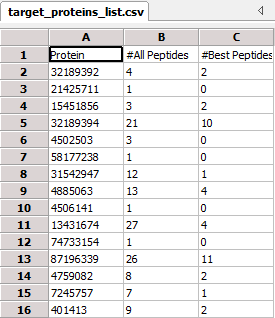
\includegraphics[scale=0.8]{Eppi_target_proteins_list}
\caption{Target\_proteins\_list table. Protein: identifier number of a target protein;\#All Peptide: number of total distinct peptides identified for a given target protein; \#Best Peptide: number of best peptides identified for a given target protein.}\label{fig:targetProtTable}
\end{center}
\end{figure}

\section{Change target peptides}
By Change Target Peptides function, the user can choose three peptides to process, changing those selected by default (\figurename~\ref{fig:change}). In fact, for each target protein, EPPI performs the database searching only for the first three peptides with best occurrence. These three peptides belong to best peptide group or to all peptide group, according to the peptide Set option in Insert Targets window (\figurename~\ref{fig:targetProt}).


\begin{figure}[htbp]
\begin{center}
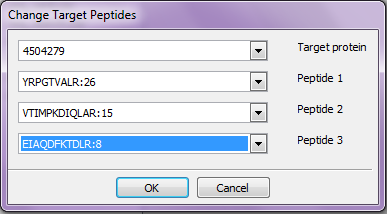
\includegraphics[scale=0.5]{Eppi_change_targets_peptides}
\caption{Change Target Peptides window. It allows to set a target protein, and three related peptides which are evaluated, as Proteotypic Peptide Set, about their capacity to target a single protein.}\label{fig:change}
\end{center}
\end{figure}

\section{Comparison by molecular weight and by amino-acid sequence}

After the comparison of each best peptide against the virtual peptidome previously created (\figurename~\ref{fig:database}), EPPI returns the number of similar peptides with indistinguishable molecular mass or amino-acid sequence. 
For each target protein, EPPI simultaneously calculate this matching for three peptides and returns the number of protein entries containing at least an indistinguishable peptide (s1, s2, s3 in \figurename~\ref{fig:card}). Furthermore, by intersecting protein subsets found (s1, s2, s3), EPPI calculates if a peptide couple or triplet improve the unambiguously identification of the target protein (s12, s23, s13, s123 in \figurename~\ref{fig:card}). For each type of comparison, by molecular weight or amino-acid sequence, the function returns three tables:
\begin{description}
\item[card.csv] reports the intersections among the protein subsets targeted by each considered peptide (best or not). 
\begin{figure}[htbp]
\begin{center}
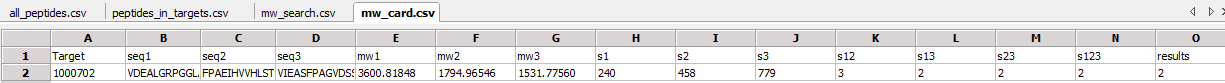
\includegraphics[scale=0.5]{card}
\caption{Card table. Seq: peptide sequence. mw: molecular weight. s1, s2, s3: number of database entries containing a peptide indistinguishable from seq1, seq2, seq3 (or mw1, mw2, mw3), respectively. s12: it indicates the number of proteins containing at least two peptides indistinguishable by both seq1 and seq2 (or mw1 and mw2); s13: it indicates the number of proteins containing at least two peptides indistinguishable by both seq1 and seq3 (or mw1 and mw3); s23: it indicates the number of proteins containing at least two peptides indistinguishable by both seq2 and seq3 (or mw2 and mw3.); s123/result: they indicate the number of proteins containing at least three peptides indistinguishable by seq1, seq2 and seq3 (or mw1, mw2 and mw3). If s123 is 0, the final result corresponds to the smaller subset (s1, s2, s3, s12, s23, s31) not empty.}\label{fig:card}
\end{center}
\end{figure}

\item[search.csv] reports, for each peptide, the number of protein entries containing similar indistinguishable peptides, by molecular weight or amino-acid sequence;
\begin{figure}[htbp]
\begin{center}
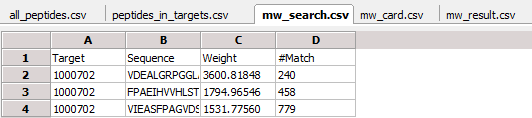
\includegraphics[scale=0.5]{search}
\caption{Search table}\label{fig:search}
\end{center}
\end{figure}
\item[result.csv] reports, for each target protein, the protein identifiers corresponding to "result" in card table (\figurename~\ref{fig:card}).
\begin{figure}[htbp]
\begin{center}
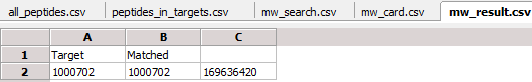
\includegraphics[scale=0.5]{result}
\caption{Result table}\label{fig:result}
\end{center}
\end{figure}
\end{description}

\section{Result and Report menu}

The result of each operation, shown in EPPI window as table, are also available as files in the folder  containing the project.   
In the drop-down menu Report (\figurename~\ref{fig:project}) are available the following functions:
\begin{description}
\item [Resume:] to show a window reporting main parameters and variable values concerning a given project; in particular, reference database used, number of processed samples/lists and number of considered proteins/peptides (\figurename~\ref{fig:report});
\item [Find protein:] to extract the sequence of a given protein, its occurrence and the occurrence of its peptides if they were experimentally identified (\figurename~\ref{fig:findP});
\item [Find a sequence:] given a peptide, it extracts the molecular weight and the corresponding parent protein. In addition, if a peptide was identified in the input files, EPPI returns its occurrence and those related to the other identified peptides for the same corresponding protein (\figurename~\ref{fig:findS}).
\end{description}

\begin{figure}[htbp]
\begin{center}
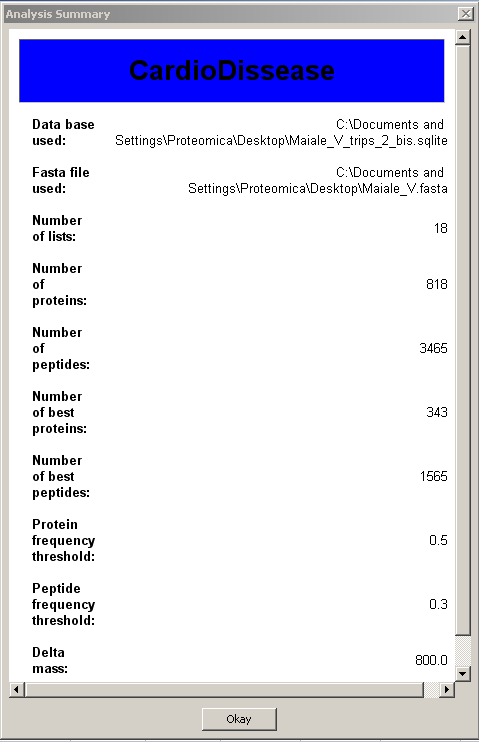
\includegraphics[scale=0.3]{Eppi_20}
\caption{Resume function result.}\label{fig:report}
\end{center}
\end{figure}

\begin{figure}[htbp]
\begin{center}
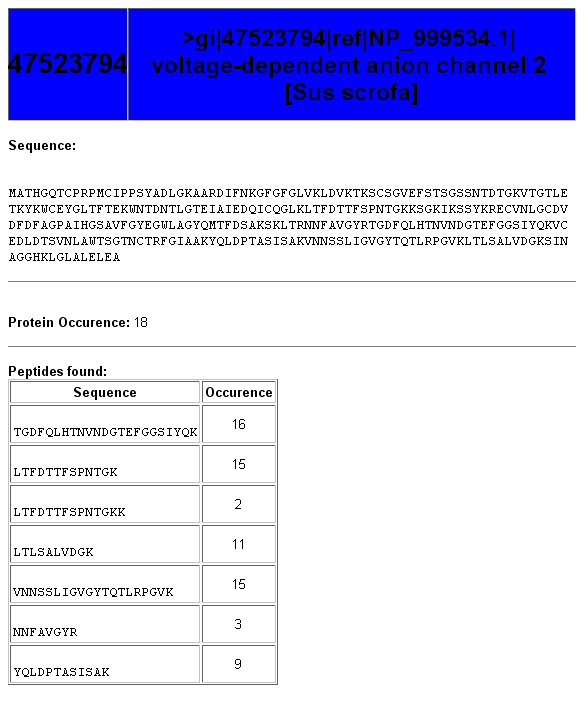
\includegraphics[scale=0.3]{Eppi_23}%
\caption{Find protein result.}\label{fig:findP}
\end{center}
\end{figure}

\begin{figure}[htbp]
\begin{center}
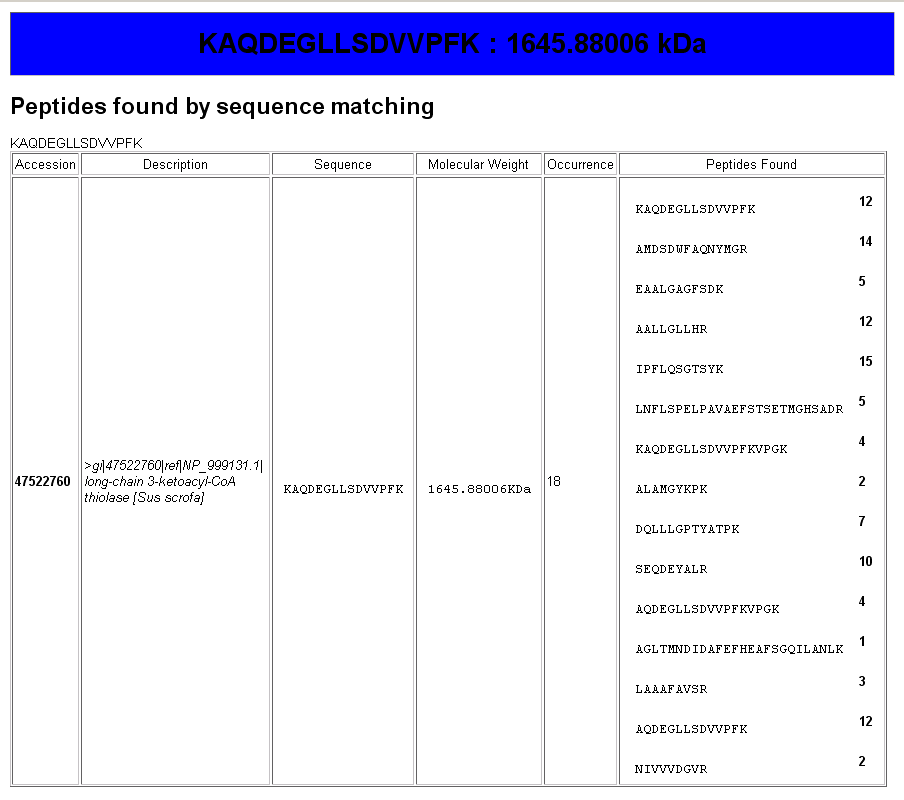
\includegraphics[scale=0.3]{Eppi_25}
\caption{Find a sequence result.}\label{fig:findS}
\end{center}
\end{figure}
 
At any time, the user can reload a previous project to consult its results, introduce or delete the input files, and also to modify the parameters used for data processing. 
\end{document}